\section{实验设计}
\subsection{Cache模块}\label{sub:Cache}
其中i\_cache模块由于无写功能无需变动,只需实现d\_cache模块的写回和写分配策略。
\subsubsection{功能描述}
Cache减少CPU访问主存的时间,提高访问速度。
\subsubsection{状态机的设计}
\begin{enumerate}
    \item 在读命中的情况下,CPU直接读取对应的cacheline的数据;
    \item 在读缺失的情况,如果索引到的cacheline是干净的,那么发送读请求,从内存读取数据,然后返回给
CPU,同时将数据写入到索引到的cacheline中;如果索引到的cacheline是脏的,那么首先要发送写
请求,将这个cacheline的脏数据写入到内存中。等待写请求处理完成后,再发送读请求,从内存中读
取对应的数据,然后再把数据返回给CPU,同时将数据写入到索引的cacheline中。
    \item 在写命中的情况下,如果索引到的cacheline是干净的,那么直接将数据写入到对应的cacheline中,
并且将dirty位置为1;如果索引到的cacheline是脏的,直接把数据写入到cache中。
    \item 在写缺失的情况下,如果索引到的cacheline是干净的,那么将数据写入到cacheline中,覆盖掉原来
的数据。如果索引到的cacheline是脏的,那么首先发送写请求,将脏的cacheline的数据更新到内存
中;然后等待第一个写请求处理完成后,然后将数据写入到索引到的cacheline中,并且将脏位标志位置为1;
\end{enumerate}
写回-写分配策略的直接映射Cache流程图如图所示:
\begin{figure}[H]
    \centering
    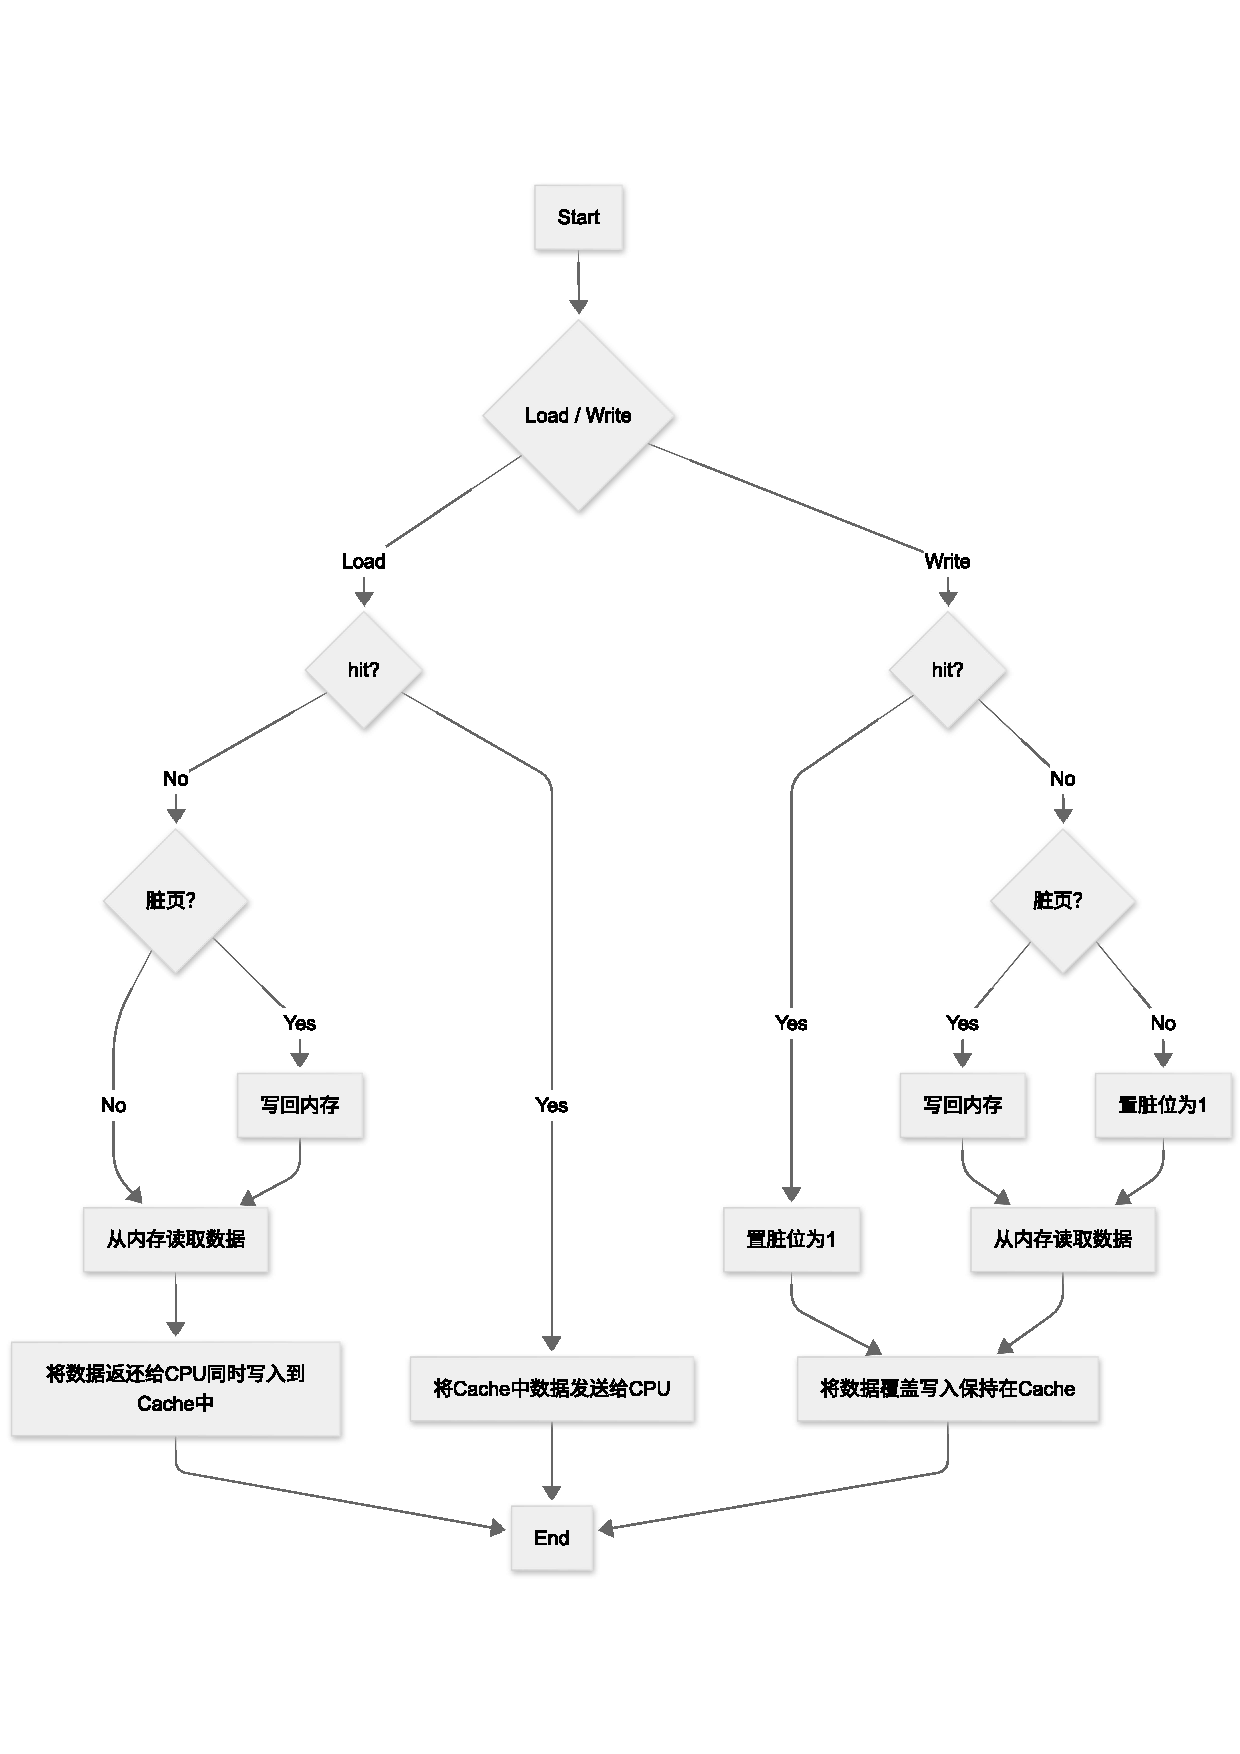
\includegraphics[width=0.75\textwidth]{image/fc.pdf}
    \caption{写回-写分配策略的直接映射Cache流程图}\label{cache_fc}
\end{figure}
写回-写分配策略的直接映射Cache状态图如图所示:
\begin{figure}[H]
    \centering
    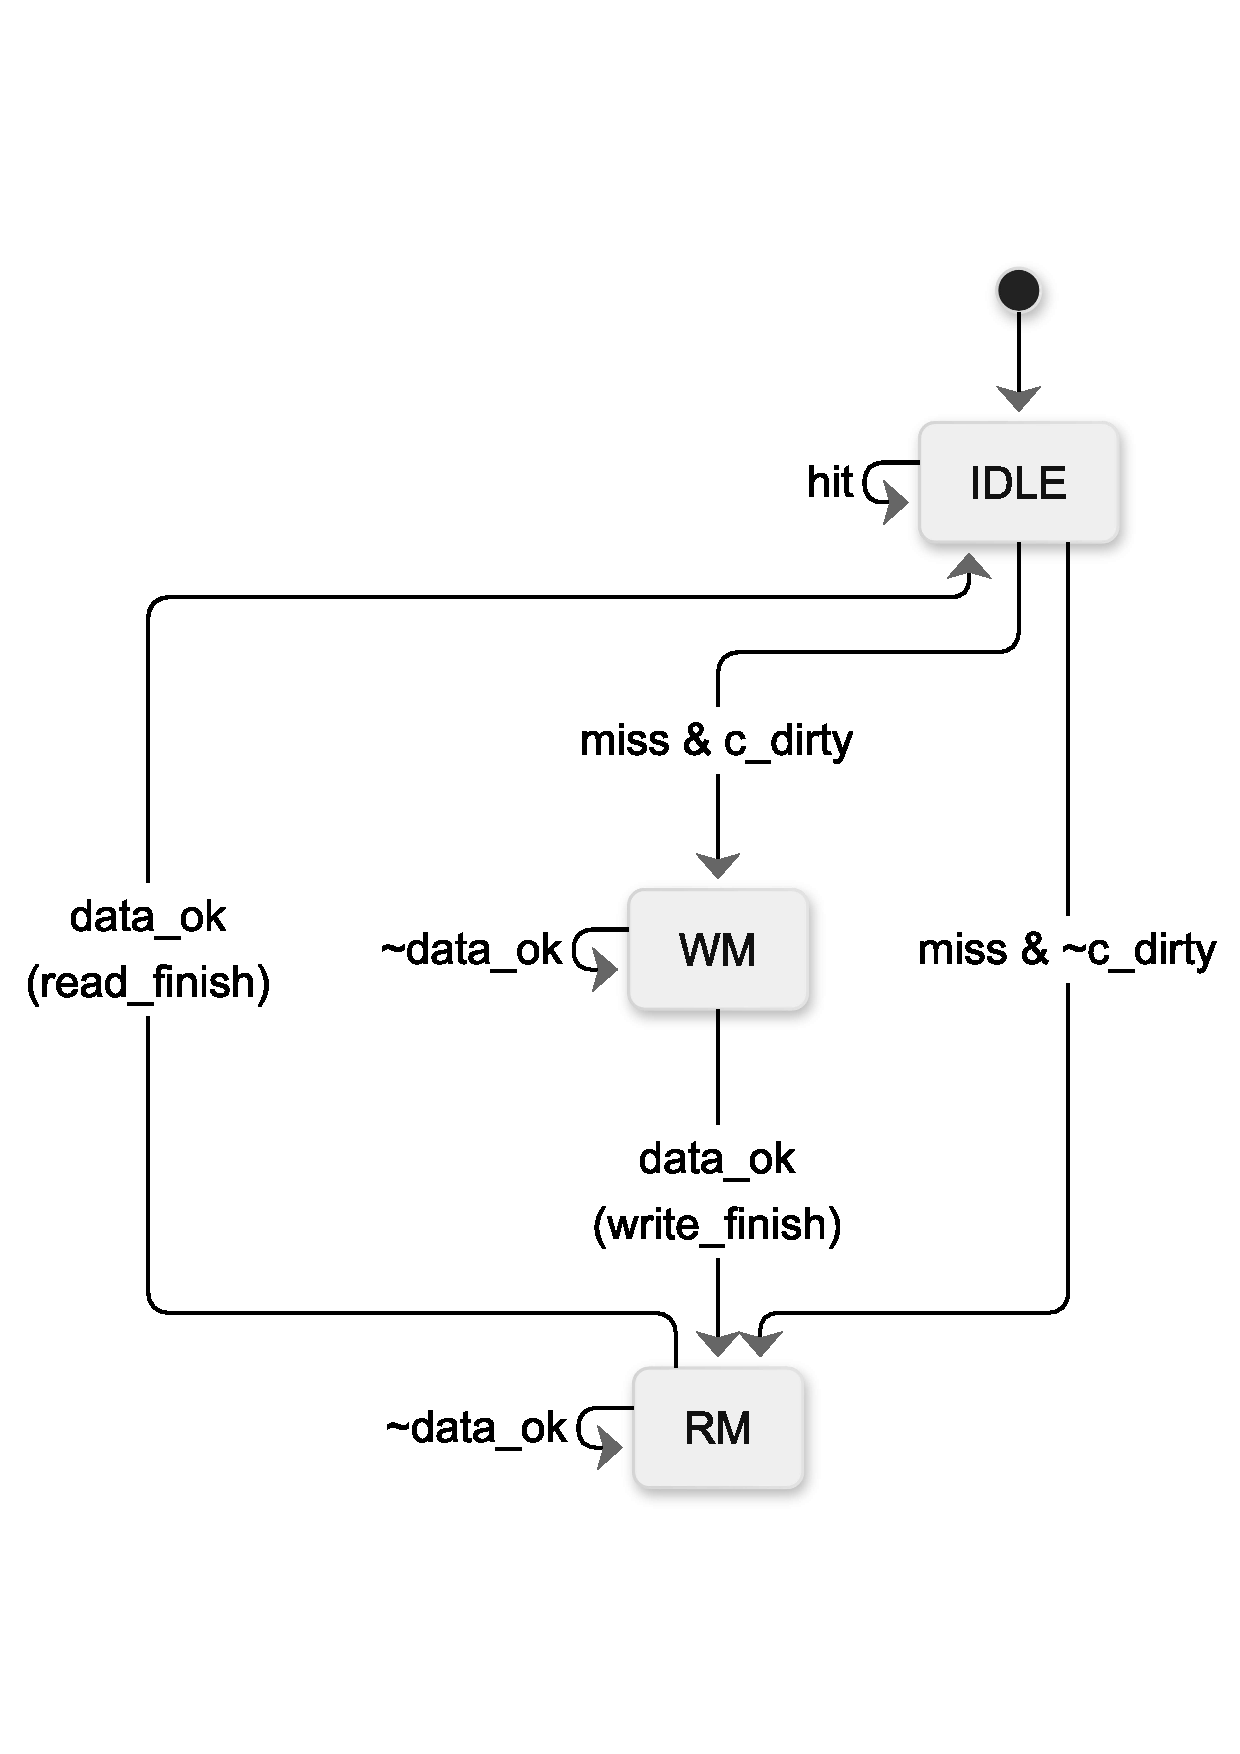
\includegraphics[width=0.5\textwidth]{image/stat.pdf}
    \caption{写回-写分配策略的直接映射Cache状态图}\label{cache_stat}
\end{figure}
\subsubsection{接口定义}
\begin{table}[H]
\centering
\caption{d\_cache 模块接口信号表}
\begin{tabular}{|l|c|c|p{7.5cm}|}
\hline
\textbf{信号名} & \textbf{方向} & \textbf{位宽} & \textbf{功能描述} \\ \hline \hline
\multicolumn{4}{|c|}{\textbf{MIPS Core 接口}} \\ \hline
\texttt{cpu\_data\_req}     & input  & 1       & MIPS CPU 请求 Cache 访问(读或写) \\ \hline
\texttt{cpu\_data\_wr}      & input  & 1       & 写使能信号,高电平表示写操作 \\ \hline
\texttt{cpu\_data\_size}    & input  & 2       & 访问字节数:00=byte,01=halfword,10/11=word \\ \hline
\texttt{cpu\_data\_addr}    & input  & 32      & CPU 发出的访存地址 \\ \hline
\texttt{cpu\_data\_wdata}   & input  & 32      & 写操作时由 CPU 提供的数据 \\ \hline
\texttt{cpu\_data\_rdata}   & output & 32      & 读操作时返回给 CPU 的数据 \\ \hline
\texttt{cpu\_data\_addr\_ok} & output & 1       & 地址阶段握手信号,表示地址接收成功 \\ \hline
\texttt{cpu\_data\_data\_ok} & output & 1       & 数据返回握手信号,表示数据有效返回 \\ \hline

\multicolumn{4}{|c|}{\textbf{AXI 接口}} \\ \hline
\texttt{cache\_data\_req}   & output & 1       & Cache 请求主存读/写数据 \\ \hline
\texttt{cache\_data\_wr}    & output & 1       & 高电平表示写请求,低电平为读请求 \\ \hline
\texttt{cache\_data\_size}  & output & 2       & 访问大小:同上 \\ \hline
\texttt{cache\_data\_addr}  & output & 32      & 发往主存的地址 \\ \hline
\texttt{cache\_data\_wdata} & output & 32      & 写回主存的数据 \\ \hline
\texttt{cache\_data\_rdata} & input  & 32      & 从主存读取回的数据 \\ \hline
\texttt{cache\_data\_addr\_ok} & input & 1     & 主存接受地址成功 \\ \hline
\texttt{cache\_data\_data\_ok} & input & 1     & 主存返回数据成功 \\ \hline
\end{tabular}
\end{table}

